\subsection{Sploty o~dwóch mostach} % (fold)
\label{sub:twobridge}
Zajmiemy się teraz związkiem supłów z indeksem mostowym.
Wiemy, że węzeł trywialny jest jednomostowy, następne w hierarchii są sploty dwumostowe.
Nazywa się je także wymiernymi, po angielsku czasami \emph{4-plats}.
Jako pierwszy studiował je Bankwitz z~Schumannem w~1934 roku.
% Kawauchi: as 4-plat presentations, which is just Conway's normal form.
Mają co najwyżej dwie składowe i~są odwracalne \cite[s. 211]{burde14}.

\begin{proposition}
    Sploty dwumostowe są pierwsze.
\end{proposition}

\begin{proof}
    Prosty wniosek z~tego, że liczba mostowa prawie jest addytywna (fakt \ref{prp:bridge_additive}).
\end{proof}

\begin{corollary}
    Węzły dwumostowe są $(\pm 2, n)$-torusowe albo hiperboliczne.
\end{corollary}

\begin{tobedone}
    % Skorzystajmy z trychotomii Thurstona: węzły dwumostowe są pierwsze, zatem nie są satelitarne.
    % Pozostało rozpatrzyć przypadek, kiedy nie są hiperboliczne.
    Teza wynika wtedy bezpośrednio z faktu \ref{prp:torus_bridge_number}, który głosi, że $br(T_{p, q}) = \min\{|p|, |q|\}$.
\end{tobedone}

\begin{proposition}
    Pierwsze węzły trzymostowe są $(\pm 3, n)$-torusowe albo hiperboliczne.
\end{proposition}

\begin{proof}
    Wniosek 10.5.2 w \cite{kawauchi96}, ale z innego twierdzenia.
\end{proof}

%\todo[inline]{Murasugi Theorem 9.3.3 (138) lub Janiak-Osajca, Pogoda (34).}
% Aus der unten stehenden Klassifikation ergibt sich, dass man jede Verschlingung mit 2 Brücken wie im Bild rechts darstellen kann, wobei {\displaystyle a_{i}\in \mathbb {Z} } a_{i}\in \mathbb{Z }  die Anzahl der Halbtwists in der jeweiligen Box bezeichnet und für gerade bzw. ungerade {\displaystyle i} i~positive {\displaystyle a_{i}} a_{i} links- bzw. rechtshändigen Halbtwists entsprechen.
% Diese Darstellung wird als Conway-Normalform bezeichnet.
% Man kann stets erreichen, dass alle {\displaystyle a_{i}} a_{i} dasselbe Vorzeichen haben.[1] Insbesondere gibt die Conway-Normalform dann ein alternierendes Knotendiagramm.[2]
%Insbesondere ist ein 2-Brücken-Knoten genau dann amphichiral, wenn {\displaystyle q^{2}\equiv -1\ mod\ p} q^{2}\equiv -1\ mod\ p ist.

\begin{proposition}
    Sploty z~dwoma mostami to dokładnie sploty typu $D(T)$ dla pewnego supła wymiernego $T$.
\end{proposition}

Dowód tego stwierdzenia znaleźć można na przykład w książce \cite{murasugi96}, strony 183-187.
Wynika z niego, że każdy splot dwumostowy można przedstawić następującym diagramem:
\[
	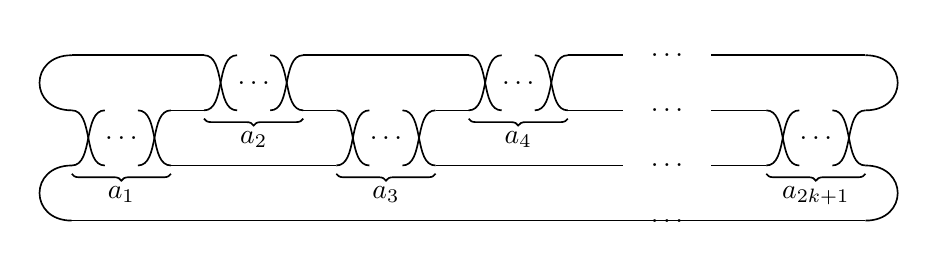
\begin{tikzpicture}[baseline=-0.65ex, xscale=0.14, yscale=0.07]
	\useasboundingbox (-40, -20) rectangle (40, 20);
		%%% A1
		\draw[semithick] (-36, -5) .. controls (-34,-5) and (-35, 5) .. (-33, 5);
		\draw[semithick] (-36,  5) .. controls (-34, 5) and (-35,-5) .. (-33,-5);
		\node at (-31.5, 0) {$\ldots$};
		\draw[semithick] (-30, -5) .. controls (-28,-5) and (-29, 5) .. (-27, 5);
		\draw[semithick] (-30,  5) .. controls (-28, 5) and (-29,-5) .. (-27,-5);
		%%% A2
		\draw[semithick] (-24,  5) .. controls (-22,  5) and (-23, 15) .. (-21, 15);
		\draw[semithick] (-24, 15) .. controls (-22, 15) and (-23,  5) .. (-21,  5);
		\node at (-19.5, 10) {$\ldots$};
		\draw[semithick] (-18,   5) .. controls (-16,  5) and (-17, 15) .. (-15, 15);
		\draw[semithick] (-18,  15) .. controls (-16, 15) and (-17,  5) .. (-15,  5);
		%%% A3
		\draw[semithick] (-12, -5) .. controls (-10,-5) and (-11, 5) .. (-9, 5);
		\draw[semithick] (-12,  5) .. controls (-10, 5) and (-11,-5) .. (-9,-5);
		\node at (-7.5, 0) {$\ldots$};
		\draw[semithick] (-6, -5) .. controls (-4,-5) and (-5, 5) .. (-3, 5);
		\draw[semithick] (-6,  5) .. controls (-4, 5) and (-5,-5) .. (-3,-5);
		%%% A4
		\draw[semithick] (0,  5) .. controls (2,  5) and (1, 15) .. (3, 15);
		\draw[semithick] (0, 15) .. controls (2, 15) and (1,  5) .. (3,  5);
		\node at (4.5, 10) {$\ldots$};
		\draw[semithick] (6,   5) .. controls (8,  5) and (7, 15) .. (9, 15);
		\draw[semithick] (6,  15) .. controls (8, 15) and (7,  5) .. (9,  5);
		%%% A 2k+1
		\draw[semithick] (27,  -5) .. controls (29,  -5) and (28, 5) .. (30, 5);
		\draw[semithick] (27, 5) .. controls (29, 5) and (28,  -5) .. (30,  -5);
		\node at (31.5, 0) {$\ldots$};
		\draw[semithick] (33,   -5) .. controls (35,  -5) and (34, 5) .. (36, 5);
		\draw[semithick] (33,  5) .. controls (35, 5) and (34,  -5) .. (36,  -5);
		%%%    - A3
		\draw[semithick] (-36, 15) to (-24, 15);
		%%% A1 - A3
		\draw[semithick] (-27, -5) to (-12, -5);
		%%% A1 - A2
		\draw[semithick] (-27,  5) to (-24,  5);
		%%% A2 - A3
		\draw[semithick] (-15,  5) to (-12,  5);
		%%% A2 - A4
		\draw[semithick] (-15, 15) to (0, 15);
		%%% A3 - A4
		\draw[semithick] (-3, 5) to (0, 5);
		%%%
		\draw[semithick] ( 9, 15) to (14, 15);
		\draw[semithick] ( 9,  5) to (14,  5);
		\draw[semithick] (-3, -5) to (14, -5);
		\node at (18,  15) {$\ldots$};
		\node at (18,   5) {$\ldots$};
		\node at (18,  -5) {$\ldots$};
		\node at (18, -15) {$\ldots$};
		\draw[semithick] (22, 15) to (36, 15);
		\draw[semithick] (22,  5) to (27,  5);
		\draw[semithick] (22, -5) to (27, -5);
		\draw[semithick] (-36, -15) to (36, -15);
		\draw[semithick] (-36, -15) [in=left,  out=left]  to (-36, -5);
		\draw[semithick] (-36,   5) [in=left,  out=left]  to (-36, 15);
		\draw[semithick] ( 36, -15) [in=right, out=right] to ( 36, -5);
		\draw[semithick] ( 36,   5) [in=right, out=right] to ( 36, 15);
		%
		\draw[semithick, decoration={brace,mirror,raise=3pt},decorate]  (-36, -5) -- node[below=4pt] {$a_1$}      (-27, -5);
		\draw[semithick, decoration={brace,mirror,raise=3pt},decorate]  (-24,  5) -- node[below=4pt] {$a_2$}      (-15,  5);
		\draw[semithick, decoration={brace,mirror,raise=3pt},decorate]  (-12, -5) -- node[below=4pt] {$a_3$}      ( -3, -5);
		\draw[semithick, decoration={brace,mirror,raise=3pt},decorate]  (  0,  5) -- node[below=4pt] {$a_4$}      (  9,  5);
		\draw[semithick, decoration={brace,mirror,raise=3pt},decorate]  ( 27, -5) -- node[below=4pt] {$a_{2k+1}$} ( 36, -5);
	\end{tikzpicture}
\]


Oto reguła, zgodnie z~którą wybieramy znaki liczb $a_i$:
jeśli $i$ jest nieparzyste, prawy skręt jest dodatni, jeśli parzyste -- lewy jest dodatni.
Sam diagram oznaczamy $C(a_1, \ldots, a_{2k+1})$ i~nazywamy postacią normalną Conwaya.

\begin{proposition}
    % Murasugi proposition 9.3.2
    Sploty dwumostowe są alternujące.
\end{proposition}

\begin{proof}
    Goodrick w~\cite{goodrick72} podał diagramatyczny dowód, gdzie ciąg ruchów zmienia diagram splotu dwumostowego w~alternujący.
    Wynika to też z faktu \ref{prp:continued_fractions}.
    % Burde, Zieschang 2013, strona 217, nazywają to twierdzeniem Bankwitza-Schumanna.
\end{proof}

Przez analogię do supłów, definiujemy ułamek łańcuchowy
\begin{equation}
    C(a_1, \ldots, a_{2k+1}) \mapsto a_1 + \frac{1}{a_2 + 1/\ldots} = \frac \alpha \beta.
\end{equation}

\begin{tobedone}
    To jest postać normalna Conwaya, ale mamy jeszcze postać Schuberta - \cite[s. 21]{kawauchi96}.
\end{tobedone}

Zauważmy, że wartość bezwzględna ułamka $\alpha/\beta$ zawsze przekracza $1$ i~odwrotnie, każdy taki ułamek pochodzi od pewnego węzła dwumostowego.
Parę względnie pierwszych liczb $(\alpha, \beta)$ nazywamy typem węzła dwumostowego.

\begin{proposition}
    \label{prp:tangle_equivalence}
    Dwumostowe sploty typów $(\alpha, \beta)$ oraz $(\alpha', \beta')$ są, pomijając orientację, równoważne wtedy i~tylko wtedy, gdy spełniony jest jeden z warunków:
    \begin{itemize}
        \item $\alpha = \alpha'$ oraz $\beta \equiv \beta' \pmod \alpha$,
        \item $\alpha = \alpha'$ oraz $\beta \beta' \equiv 1 \pmod \alpha$.
    \end{itemize}
\end{proposition}

% Burde, Zieschang 2013: strona 212, dowód tego.

\begin{tobedone}
    \cite[s. 23]{kawauchi96}: czasem $2\alpha$ zamiast $\alpha$.
\end{tobedone}

\begin{proof}
    Dowód opiera się na tym, że podwójnie cykliczna przestrzeń nakrywająca rozcięta wzdłuż splotu jest przestrzenią soczewkową typu $(\alpha, \beta)$.
    Nie definiowaliśmy nawet tych przestrzeni, szczegóły można znaleźć w~podręczniku \cite{murasugi96} albo \cite{schubert56}.
\end{proof}

\begin{proposition}
    Dwumostowy splot typu $(\alpha, \beta)$ jest achiralny dokładnie wtedy i tylko wtedy, gdy
    \begin{equation}
        \beta^2 \equiv -1 \mod \alpha.
    \end{equation}
\end{proposition}

\begin{proof}
    Wynika to z tego, że lustrem splotu typu $(\alpha, \beta)$ jest splot typu $(\alpha, -\beta)$ oraz faktu \ref{prp:tangle_equivalence}.
\end{proof}

\begin{proposition}
    Niech $b$ będzie dowolną liczbą całkowitą.
    Wtedy następujące sploty są tego samego typu:
    \begin{align}
        N(T(a_1, a_2, \ldots, a_{2k+1})) & \approx N(T(a_1, a_2, \ldots, a_{2k+1}, b, 0)) \\
                                         & \approx D(T(-a_1, -a_2, \ldots, -a_{2k+1}, b)) \\
                                         & \approx C(a_1, a_2, \ldots, a_{2k}-1, 1). \\
        N(T(a_1, a_2, \ldots, a_{2k}))   & \approx D(T(-a_1, -a_2, \ldots, -a_{2k}, b)) \\
                                         & \approx C(a_1, a_2, \ldots, a_{2k}-1, 1). \\
        D(T(a_1, a_2, \ldots, a_{2k+1})) & \approx D(T(a_1, a_2, \ldots, a_{2k}, 0)) \\
                                         & \approx C(1, a_1-1, a_2, \ldots, a_{2k}). \\
        D(T(a_1, a_2, \ldots, a_{2k}))   & \approx D(T(a_1, a_2, \ldots, a_{2k-1}, 0)) \\
                                         & \approx C(a_1, a_2, \ldots, a_{2k-1}).
    \end{align}
\end{proposition}

\begin{proof}
    \cite[fakt 9.3.4]{murasugi96}
\end{proof}

\begin{proposition}
    Niech $L$ będzie dwumostowym splotem typu $(\alpha, \beta)$.
    Wtedy $\det L = \alpha$.
\end{proposition}

Wynika stąd, że wyznacznik nie wystarcza do odróżniania splotów dwumostowych.

\begin{proof}
    % Chcąc oszczędzić niektórym Czytelnikom cierpień odsyłamy po prostu do \cite{schubert56}.
    \url{https://math.stackexchange.com/questions/3327846/}.
\end{proof}

Niech $A, B$ będą supłami.
Wiemy, że suma $A+B$ nie musi być supłem, zaś $D(A+B)$ niekoniecznie jest splotem dwumostowym.
Pomimo to, splot $N(A+B)$ jest dwumostowy, potrafimy nawet powiedzieć, jaki ma wyznacznik:

\begin{proposition}
    % Theorem 9.3.5 Murasugi

    Niech $A, B$ będą supłami, którym odpowiadają skrócone ułamki $p/q$ oraz $r/s$.
    Wtedy splot $L = N(A+B)$ jest dwumostowy, typu $(\alpha, \beta)$ i ma wyznacznik $\alpha = |ps + qr|$.
\end{proposition}

Murasugi (twierdzenie 9.3.5) twierdzi, że dowód znajduje się w \cite{ernst90}.

\begin{proposition}
    Rozpatrzmy węzeł dwumostowy typu $(\alpha, \beta)$, gdzie $0 < \beta < \alpha$ i~$\beta$ jest nieparzyste.
    Niech $r_k$ będzie resztą z~dzielenia $k\beta$ przez $2\alpha$ leżącą w~przedziale $(-\alpha, \alpha)$ dla $k = 0, 1, \ldots, \alpha - 1$.
    Różnica między ilością dodatnich reszt i~ujemnych reszt to sygnatura węzła.
\end{proposition}

Wygląda na to, że jedynym niewyznaczonym do końca klasycznym niezmiennikiem jest liczba gordyjska.

% Koniec podsekcji Sploty o~dwóch mostach
